\documentclass[]{article}
\usepackage[utf8]{inputenc}
\usepackage[spanish]{babel}
\usepackage[margin=2cm]{geometry}
\usepackage{amsmath}
\usepackage{graphicx}
\usepackage{booktabs}
\usepackage{}

\title{Tarea 2: Sistemas Equivalentes \\ [0.5em] \large ICE2006 - 1}
\author{Agustin Bustamante}


\begin{document}

\maketitle

\newpage

\section{Introduccion y Objetivos}
Este informe presenta la resolución de problemas de estática relacionados a fuerzas distribuidas, cálculos de centros de masa y sistemas equivalentes tanto para 2D como para 3D, para esto se utilizó el lenguaje de programación Python. El presunto informe se enfoca en el análisis de componentes mecánicos y estructuras con grandes cantidades de datos.

los principales objetivos de este informe son:
\begin{itemize}
	\item Representación de fuerzas distribuidas mediante fuerzas puntuales equivalentes sobre estructuras de reticulados.
	\item Calculo de áreas y centroides de múltiples superficies mediante el teorema de Green-Stokes.
	\item Determinar masa y centro de masa de un sistema con densidad variable.
	\item Analizar el efecto que genera la presión del viento en estructuras tridimensionales, a través de cálculos de sistemas equivalentes de fuerza y momento.
\end{itemize}

\section{Marco Teórico}
\subsection{Fuerza Distribuidas en reticulados}
Para el análisis estructural, representamos las cargas distribuidas sobre las barras como fuerzas puntuales equivalentes aplicadas en ambos nodos. Una carga uniforme $q$ sobre un elemento con longitud $L$ genera una fuerza tal que
\begin{equation}
	F_{eq} = q \cdot L
\end{equation}
Esta fuerza se distribuye de manera equitativa entre los nodos del elemento con el fin de mantener la equivalencia estática.

\subsection{Geometría polígonos}
Para polígonos bidimensionales de $N$ lados conocidos, el área y centroide pueden ser calculados a través de sumatorias las cuales relacionan las coordenadas de vértices consecutivos:

\begin{itemize}
	\item Área (A):
\begin{equation}
	1/2\sum_{i=1}^{N} (x_iy_{i+1} - x_{i+1}y_i)
\end{equation}
	\item Centroide (x, y):

\begin{equation}
	x = 1/{6A}\sum_{i=1}^{N} (x_i + x_{i+1})(x_iy_{i+1} - x_{i+1}y_i)
\end{equation}

\begin{equation}
	y = 1/{6A}\sum_{i=1}^{N} (y_i + y_{i+1})(x_iy_{i+1} - x_{i+1}y_i)
\end{equation}

\end{itemize}

\subsection{Centro de Masa y Sistemas Compuestos}
En sistemas que se componen por una múltiple cantidad de polígonos con densidades variables dependientes de su respectivo polígono $(P_i)$ sabemos que la masa total del sistema $(M_t)$ y su centro de masa respectivo $(X_{ct})$ donde $X_{ct}$ resultan de ponderaciones de propiedades individuales:
\begin{itemize}
	\item Masa Total del sistema $(M_t)$:
\begin{equation}
	M_t = \sum(P_i \cdot A_i)
\end{equation}
	
	\item Posición centro de masa $(X_{ct})$:
\begin{equation}
	M_t = \sum(m_i \cdot x_i)
\end{equation}
\end{itemize}

\subsection{Presión del viento y cargas en 3D}
La presión del viento $P$ varía en función de la altura $z$ siguiendo las ecuaciones:
\begin{equation}
	v(z) = v_0(z/h)^a\alpha
\end{equation}

\begin{equation}
	P(v) = 0,613 \cdot v(z)^2
\end{equation}
Teniendo en consideración que para la resultante de fuerza emitida en un área por la presión es considerada unicamente la componente del viento que siga la recta del vector normal a la superficie, y solamente si este posee símbolo opuesto en su componente de x a la normal del plano

\section{Presentación de Resultados}
\subsection{Problema 1: Torsor Estructura Reticulado}
\begin{table}[htbp]
	\centering
	\caption{Torsor equivalente sistema Problema 1}
	\label{tab: resultados Torsor}
	\begin{tabular}{lccc}
		\toprule
		\textbf{caso} & $\vec{R}$ (\text{N}) & $\vec{M}_t$ (\text{N m}) & $\vec{X}$ (\text{m}) \\
		\midrule
		Sistema 1 & (150, -1330, 0) & (0, 0, 0) & (5.263, 0, 0) \\
		\bottomrule
	\end{tabular}
\end{table}

\begin{figure}[htbp]
	\centering
	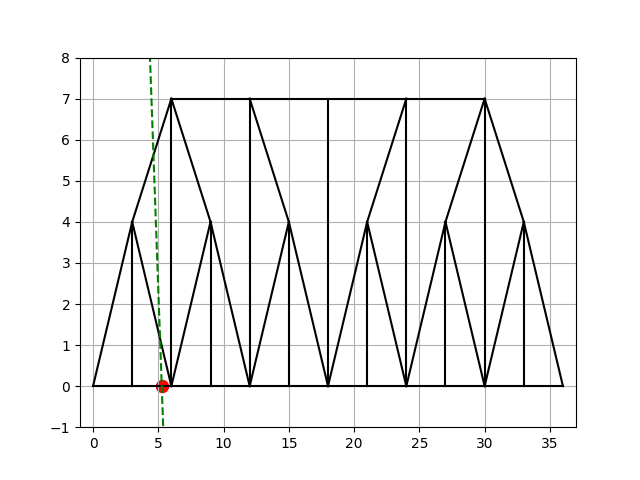
\includegraphics[width=0.6\textwidth]{EstructurareticuladoP1.png}
	\caption{Representacion reticulado, con recta de torsor equivalente}
	\label{fig:reticulado_P1}
\end{figure}

\subsection{Problema 2: }
\begin{table}[htbp]
	\centering
	\caption{Resultados internos estructura Problema 2}
	\label{tab: Res_pt1_P2}
	\begin{tabular}{lcccc}
		\toprule
		\textbf{sistema} & $A_t$ (\text{$m^2$}) & $\vec{X}_{cen}$ (\text{m}) & ${M}_t$ (\text{Kg}) & $X_{ct}$\\
		\midrule
		Sistema 2 & 1043.792 & (18.829, 20.096, 0) & 311.413 & (0.001, 0.005, 0) \\
		\bottomrule
	\end{tabular}
\end{table}

\begin{table}[htbp]
	\centering
	\caption{Resultados Cargas aplicadas Problema 2}
	\label{tab: Res_pt2_P2}
	\begin{tabular}{lcc}
		\toprule
		\textbf{sistema} & $\vec{R}$ (\text{N}) & $\vec{Pos}$ (\text{m}) \\
		\midrule
		Sistema 2 & (0, 0, -120.609) & (14.228, 21.737, 0) \\
		\bottomrule
	\end{tabular}
\end{table}
\begin{figure}[htbp]
	\centering
	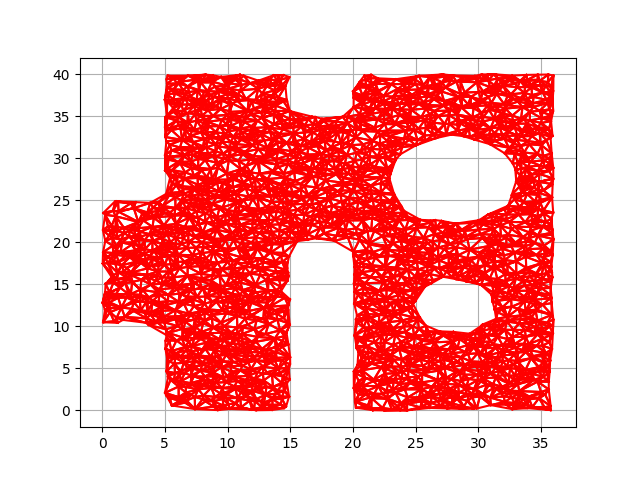
\includegraphics[width=0.6\textwidth]{EstructurareticuladoP2.png}
	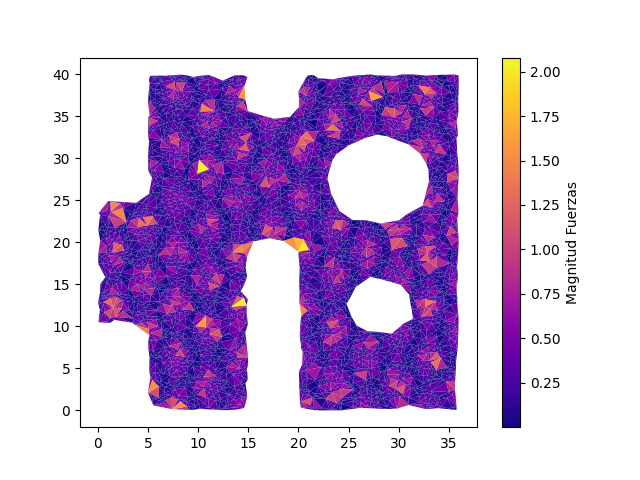
\includegraphics[width=0.6\textwidth]{mapacalorP2.png}
	\caption{Representacion reticulado y mapa de calor Problema 2}
	\label{fig:reticulado y mapa calor P2}
\end{figure}

\begin{table}[htbp]
	\centering
	\caption{Resultados internos estructura Problema 2}
	\label{tab: Res_pt1_P2}
	\begin{tabular}{l}
		\toprule
		\textbf{Indice elemento sometido a mayor fuerza}\\
		\midrule
		\textbf{5275}\\
		\bottomrule
	\end{tabular}
\end{table}
\end{document}